\documentclass{article}
\usepackage{proof}
\usepackage{bussproofs}
\usepackage{xcolor}
\usepackage{url}
\usepackage{framed}
\usepackage{amsmath, amsfonts, amssymb}
\usepackage{mathtools}
\usepackage{minted}
\usepackage{stmaryrd}
\usepackage{verbatim}
\usepackage{graphicx}
\usepackage{hyperref}

\hypersetup{
 pdfborder={0 0 0},
 colorlinks=true,
 linkcolor=blue,
 urlcolor=blue,
 citecolor=blue
}
\usepackage{cleveref}


\newcommand{\rem}[1]{\textcolor{red}{[#1]}}
\newcommand{\ed}[1]{\textcolor{blue}{#1}}
\newcommand{\ct}[1]{\rem{#1 --ct}}

\begin{document}
\title{Comprehensive Exam Report 2 - Relating Higher Order and First-Order Logics}
\author{Arjun Viswanathan}
\date{}
\maketitle

\section{Introduction}
\label{sec:intro}
	In this report, we will discuss the 
	integration of automatic theorem provers 
	(ATPs) with interactive theorem 
	provers (ITPs). We will particularly
	focus on the ATP category of 
	satisfiability modulo theories (SMT) 
	solvers. ITPs are highly 
	reliable tools with a small proof kernel. 
	They require the user to write elaborate 
	proofs to formalize properties, and 
	provide little automation. ATPs, on the 
	other hand automatically prove formulas
	without any user intervention.  
	Users would benefit from having 
	the reliability of ITP results 
	with the automation capabilities
	of ATPs. However, SMT solvers have an 
	enormous code base, and due to the 
	lack of a small, verifiable kernel, 
	are susceptible to bugs. Thus, in a 
	collaboration with an SMT 
	solver, an ITP's trust-base would be 
	extended to include the solver's. To 
	avoid compromising the proof kernel of 
	the ITP, SMT solvers can 
	produce proofs of their results. 
	We explore how proof producing 
	SMT solvers can guide ITPs in 
	finding proofs for formulas - 
	a process called \textit{proof 
	search}. To assist ITPs in automation
	of proof search, the proof object from 
	the SMT solver guides the proof search 
	in the ITP via a process called
	\textit{proof reconstruction}.
	Reconstruction can be implemented 
	as a meta-procedure. For example, 
	reconstruction of SMT solver proofs 
	in Isabelle/HOL are done external to 
	the prover's logic~\cite{bohme}.
	Here, the external ATP's proof guides 
	\textit{Metis}, Sledgehammer's
	internal ATP in its proof search.
	The final proof is found by 
	\textit{Metis} and the SMT solver's 
	proof is only used to prune the 
	search space, and fill in holes.
	In SMTCoq~\cite{DBLP:phd/hal/Keller13},
	this reconstruction is 
	expressed within the ITP's logic 
	by a process called 
	\textit{computational reflection}.
	Here, the SMT solver's logic is 
	embedded in Coq's logic, and then 
	a proof from the SMT solver is 
	directly used to obtain the 
	proof of a formula in Coq. 
	While this reduces the 
	proof obligation within Coq, it incurs
	an overhead of checking the SMT 
	solver's proof, which is typically 
	large, inside Coq, making it a
	potentially time consuming process. 
	We look in detail into both these 
	approaches of integrating SMT solvers 
	with ITPs.
	
\section{Preliminaries}
\label{sec:prelims}
	First-order logic\\
	Clauses as sets\\
	Coq lists [] and coq arrays \{\}.

\section{SMTCoq}
\label{sec:smtcoq}
	SMTCoq is a skeptical cooperation 
	between the Coq proof assistant, and 
	SAT and SMT solvers, implemented as a 
	Coq plugin. We will maintain a focus 
	on the SMT solver integration of 
	SMTCoq, noting that most features are 
	shared with the SAT	solver integration.
	
	\begin{figure}
		\begin{framed}
			\textsc{Step 1}: Coq calls SMTCoq over 
			a Boolean formula $F$:
			\begin{minted}{Coq}
Theorem F : forall (a b c : bool), (b && negb c) || 
  (a && negb b) || negb a || c = true.
Proof.
  smt.
			\end{minted}
		\end{framed}
		
		\begin{center}
			$\big\downarrow$
		\end{center}
		
		\begin{framed}
			\begin{center}
				\textsc{Step 2}: SMT solver 
				proves $F$ and returns proof 
				\texttt{t}. This step is 
				expanded in Fig.~\ref{fig:smtex}
			\end{center}
		\end{framed}
		
		\begin{center}
			$\big\downarrow$
		\end{center}
		
		\begin{framed}
			\textsc{Step 3}: SMT Coq's checker 
			checks deep embedding of $F$, 
			\texttt{f}, against proof 
			\texttt{t}:
			\begin{center}
				\texttt{checker f t = true}
			\end{center}
		\end{framed}
		
		\begin{center}
			$\big\downarrow$
		\end{center}
		
		\begin{framed}
			\textsc{Step 4}: Reflection principle 
			reflects deep embedding to shallow 
			embedding $\mathbb{I}(\texttt{f})$:
			\begin{center}
				\texttt{checker\_correct f t 
					(refl\_equal (checker 
					f t) true)}
			\end{center}
		\end{framed}
		
		\begin{center}
			$\big\downarrow$
		\end{center}
		
		\begin{framed}
			\textsc{Step 5}: Proof of $F$ is 
			completed in Coq:
			\begin{minted}{Coq}
Theorem F : forall (a b c : bool), (b && negb c) || 
  (a && negb b) || negb a || c = true.
Proof.
  smt.
Qed.
			\end{minted}
		\end{framed}
		
		\caption{SMTCoq's journey in proving 
			example Boolean formula $F$}
		\label{fig:smtcoqex}
	\end{figure}

	ATPs like SMT solvers are susceptible 
	to bugs due to the large code-bases 
	used to support	their automation. 
	ITPs like Coq have a small trustable 
	proof kernel which would be 
	compromised if they were to trust
	external results. In a collaboration
	with SMT solvers, to avoid extending 
	Coq's trust-base, SMTCoq requires the 
	solvers to be proof-producing, and uses 
	Coq's computational capabilities 
	to lift their proofs up to Coq proofs, 
	in a process called computational 
	reflection. This is illustrated in 
	Fig.~\ref{fig:smtcoqex} using a 
	running example that is elaborated 
	in the rest of the section.

	\begin{figure}[t]
		\begin{framed}
			\textsc{Step 2.1}: $F$ is negated:
			\begin{align*}
				F&: (b \land \neg c) \lor 
				(a \land \neg b) \lor \neg a 
				\lor c\\
				\neg F&: \neg((b \land \neg c) 
				\lor (a \land \neg b) \lor \neg 
				a \lor c)
			\end{align*}
		\end{framed}
		
		\begin{center}
			$\big\downarrow$
		\end{center}
		
		\begin{framed}
			\textsc{Step 2.2}: $\neg F$ after CNF 
			conversion is checked for 
			unsatisfiability by the SMT solver:
			\begin{align*}
				&\{\neg b \lor c, \neg a \lor b,
				a, \neg c\}
			\end{align*}
		\end{framed}
		
		\begin{center}
			$\big\downarrow$
		\end{center}
		
		\begin{framed}
			\textsc{Step 2.3}: SMT solver produces 
			proof \texttt{t} of 
			unsatisfiability of $\neg F$ or of
			validity of $F$:
			\begin{prooftree}
				\AxiomC{$\neg c$}
				\AxiomC{$\neg b \lor c$}
				\AxiomC{$\neg a \lor b$}
				\BinaryInfC{$\neg a \lor c$}
				\AxiomC{$a$}
				\BinaryInfC{$c$}
				\BinaryInfC{$\bot$}
			\end{prooftree}
		\end{framed}
	
		\caption{The SMT Solver's role in 
			helping SMTCoq prove example 
			formula $F$.}
		\label{fig:smtex}
	\end{figure}

	SMT solvers refutationally prove 
	input formulas --- given a formula
	$F$, the solver proves that the 
	negation of $F$ ($\neg F$) is 
	unsatisfiable, which is equivalent
	to proving that $F$ is valid. 
	To do this, the SMT solve converts 
	$\neg F$ into conjunction or clausal 
	normal form (CNF) which is a 
	conjunction of clauses (disjunctions 
	of literals). It then uses 
	a combination of a SAT solver and 
	multiple theory	solvers to reduce 
	the set of input clauses to the 
	empty clause via resolution
	and other rules of inference. Thus,
	deriving the empty clause, which 
	represents $False$, from the input 
	clauses proves that the input clauses 
	are unsatisfiable. A proof
	from an SMT solver is a tree 
	with the input clauses (from the 
	negation of the input formula) at
	the leaves and the empty clause
	at the root. The role of the SMT
	solver from Fig.~\ref{fig:smtcoqex}
	is elaborated in Fig.~\ref{fig:smtex}.
	The SMT solver's proof creation is 
	detailed in Report 3.
	
	SMTCoq implements a checker for 
	SMT solver proofs (Step 3). It 
	encodes the language of SMT solvers
	in Coq as two different embeddings. 
	Given a logical framework A, and 
	a logical framework B, in which we 
	want to represent the language of A, 
	there are two ways to achieve this
	representation, and 
	both of these are necessary for 
	reflection:
	\begin{itemize}
		\item \textit{Shallow Embedding: }
		Use types and terms of B that 
		correspond to those of A, to 
		represent terms of A. A shallow
		embedding of SMT formulas in 
		Coq is Coq's \texttt{bool} 
		type of Booleans.
		\item\textit{Deep Embedding: }
		Define custom types in B that 
		correspond to those of A, and 
		define inside B, the meaning of 
		terms of these custom types with 
		respect to shallow terms. A 
		deep embedding of SMT formulas 
		is defined as the type 
		\texttt{form} in SMT solvers.
		\texttt{f} from 
		Fig.~\ref{fig:smtcoqex} has
		type \texttt{form}.
	\end{itemize}

	Given formula $F$, SMTCoq's proof 
	checker checks the deep embedding of 
	$F$ against the proof of $F$ from the 
	SMT solver. If the checker succeeds, 
	SMTCoq is able to reflect the formula in 
	the deep embedding to its shallow 
	embedding. This is done via a 
	correctness lemma for the checker
	(also called the reflection principle),
	which proves that for any 
	formula in the deep embedding, if 
	the checker is able to check an SMT
	proof against it, then the formula in 
	the shallow embedding is true. A 
	proof of $F$ in the shallow 
	embedding is obtained by instantiating 
	the correctness lemma with $F$.
	Step 4 shows the instantiation of 
	the reflection principle with 
	the right objects to obtain the 
	proof of our example formula 
	from Fig.~\ref{fig:smtcoqex}. 
	The interpretation function
	$\mathbb{I}$ transforms 
	formulas in the deep embedding
	to their shallow embeddings
	given a valuation of the free 
	variables $\nu$, so 
	$\forall\ \nu,\ 
	\mathbb{I}_{\nu}(\texttt{f})$
	is exactly the proof required 
	to close theorem $\texttt{F}$
	in Coq. The reflection principle 
	is explained in the next section.	
	
	SMTCoq is \textit{sound} ---
	when it proves a formula in Coq, the 
	formula is valid and thus the proof
	can be closed (using \texttt{Qed.},
	as in Fig.~\ref{fig:smtcoqex}), but 
	not \textit{complete} --- when it 
	fails to prove a formula, we can't 
	be certain that the formula isn't 
	valid. This is because, the underlying 
	SMT solver cannot decide certain 
	formulas - given a formula, it could 
	either return \texttt{sat} 
	(satisfiable), \texttt{unsat} 
	(unsatisfiable), or 
	\texttt{unknown} (`don't know').
	Additionally, SMTCoq only works for 
	quantifier-free SMT logics. The 
	SMT theories it currently supports 
	are the theories of equality over
	uninterpreted functions (EUF), 
	liniear integer arithmetic (LIA),
	bit-vectors (BV), and arrays with
	extensionality (AX).
	
	\subsection{Checker}
	\label{sec:checker}
	SMTCoq's checker checks the deep embedding
	of SMT formulas in Coq against the 
	proof trees discharged by the SMT solver.
	Recall that a deep embedding is an
	inductive type written in 
	Coq representing SMT formulas. 
	In the following, we present 
	a simplified version of SMTCoq's 
	deep embedding. The actual embedding 
	uses Coq's machine integers to 
	implement sharing of terms and 
	optimize space, but an unoptimized 
	and simpler version is presented 
	below. 
	
	\texttt{form} is the type of 
	formulas:
	\begin{minted}{coq}
Inductive form : Type :=
 | Fatom (_ : atom)
 | Ftrue
 | Ffalse
 | Fnot (_ : form)
 | Fand (_ : array form)
 | For (_ : array form)
 | Fimp (_ : array form)
 | Fxor (_ _ : form)
 | Fiff (_ _ : form)
 | Fite (_ _ _ : form)
	\end{minted}
	where a formula can be an atom, 
	\texttt{true}, \texttt{false};
	a negation of a formula; a 
	conjunction, disjunction, or 
	implication of two or more 
	formulas; an exclusive-or or
	an equivalence of two formulas; 
	or, an if-then-else of three formulas.
	\texttt{atom} is the type of atoms
	or terms:
	\begin{minted}{Coq}
Inductive atom : Type :=
 | AppIntr (_ : op) (_: list atom)
 | AppUnintr (_ : int) (_: list atom).	
	\end{minted} 
	which can be applications of 
	either interpreted functions 
	(from a theory) or uninterpreted
	functions to zero (constants) or more 
	terms. Uninterpreted constants 
	are parameterized by machine 
	integers while interpreted ones 
	are encoded as follows:
	\begin{minted}{Coq}
Inductive op : Type :=
 | Zcst (_ : Z) | Zle | Zlt | Zplus | ...
 | Eq (_ : type).
	\end{minted}
	Some of the interpreted integer 
	functions are shown in \texttt{op}.
	Similarly, there are interpreted 
	functions from each theory.
	Some examples of atoms are 
	\begin{itemize}
		\item \texttt{AppUnintr 0 [AppUnintr 
			1 []]} for the term $f(x)$ where 
			$f$ has index $0$, and $x$ has 
			index $1$; 
		\item \texttt{AppIntr Zplus [(AppIntr 
			(Zcst 5) []); (AppUnintr 2 [])]} 
			for the term $5 + y$ where $y$ 
			has index $2$.
		\item Recursively, from the previous example,
			\texttt{AppUnint 
			1 []} for $x$.
		\item Recursively, from the previous example,
			\texttt{AppUnint 2 []} for $y$.
	\end{itemize}
	Finally, for convenience of representing 
	CNF formulas in SMTCoq, a \texttt{clause} 
	data structure encodes a disjunction of 
	literals as a list of its constituents 
	and a \texttt{state} represents the entire 
	formula in CNF as an array of the 
	respective conjuncts. Thus, the deep 
	embedding of formula $F$ from our running 
	example, is the encoding of the set 
	$\{\neg b \lor c, \neg a \lor b, a, 
	\neg c\}$ from step 2.2 of 
	Fig.~\ref{fig:smtex} 
	as the following \texttt{state}:
	\begin{align*}
		\{&\texttt{[Fnot Fatom (AppUnint 1 []); 
				  Fatom (AppUnint 2 [])],} &(*\ \neg b \lor c\ *)\\
		  &\texttt{[Fnot Fatom (AppUnint 0 []);
				  Fatom (AppUnint 1 [])],} &(*\ \neg a \lor b\ *)\\
		  &\texttt{[Fatom (AppUnint 0 [])],
				  [Fnot Fatom (AppUnint 2 [])]}\} &(*\ a, \neg c\ *)  
	\end{align*}
	where $a, b,$ and $c$ are indexed as 
	$0, 1,$ and $2$.
	
	The checker inputs a formula in its 
	deep embedding, and a proof of the 
	formula from the SMT solver, and 
	returns \texttt{true} if the proof 
	proves the formula, and 
	\texttt{false} otherwise:
	\begin{center}
		\texttt{checker (f : 
			form) (t : T) : bool}	
	\end{center}
	Although all SMT solvers provide a
	refutation tree as a proof, as 
	illustrated step 2.3 of 
	Fig.~\ref{fig:smtex},
	their proof formats vary. CVC4 uses 
	LFSC~\cite{DBLP:journals/fmsd/StumpORHT13}
	which is a meta-logic that allows the 
	specifying of proof calculi that have 
	declarative	rules with computational 
	components called side conditions, and 
	veriT uses a proof language similar to 
	SMTLIB~\cite{Besson1}. SMTCoq has its 
	own proof certificate format for SMT 
	solver proofs and it translates proofs 
	from all formats to this format, 
	and \texttt{T} is the type of 
	these certificates that are 
	checked by the checker. 
	
	\begin{figure}[t]
	\begin{center}
	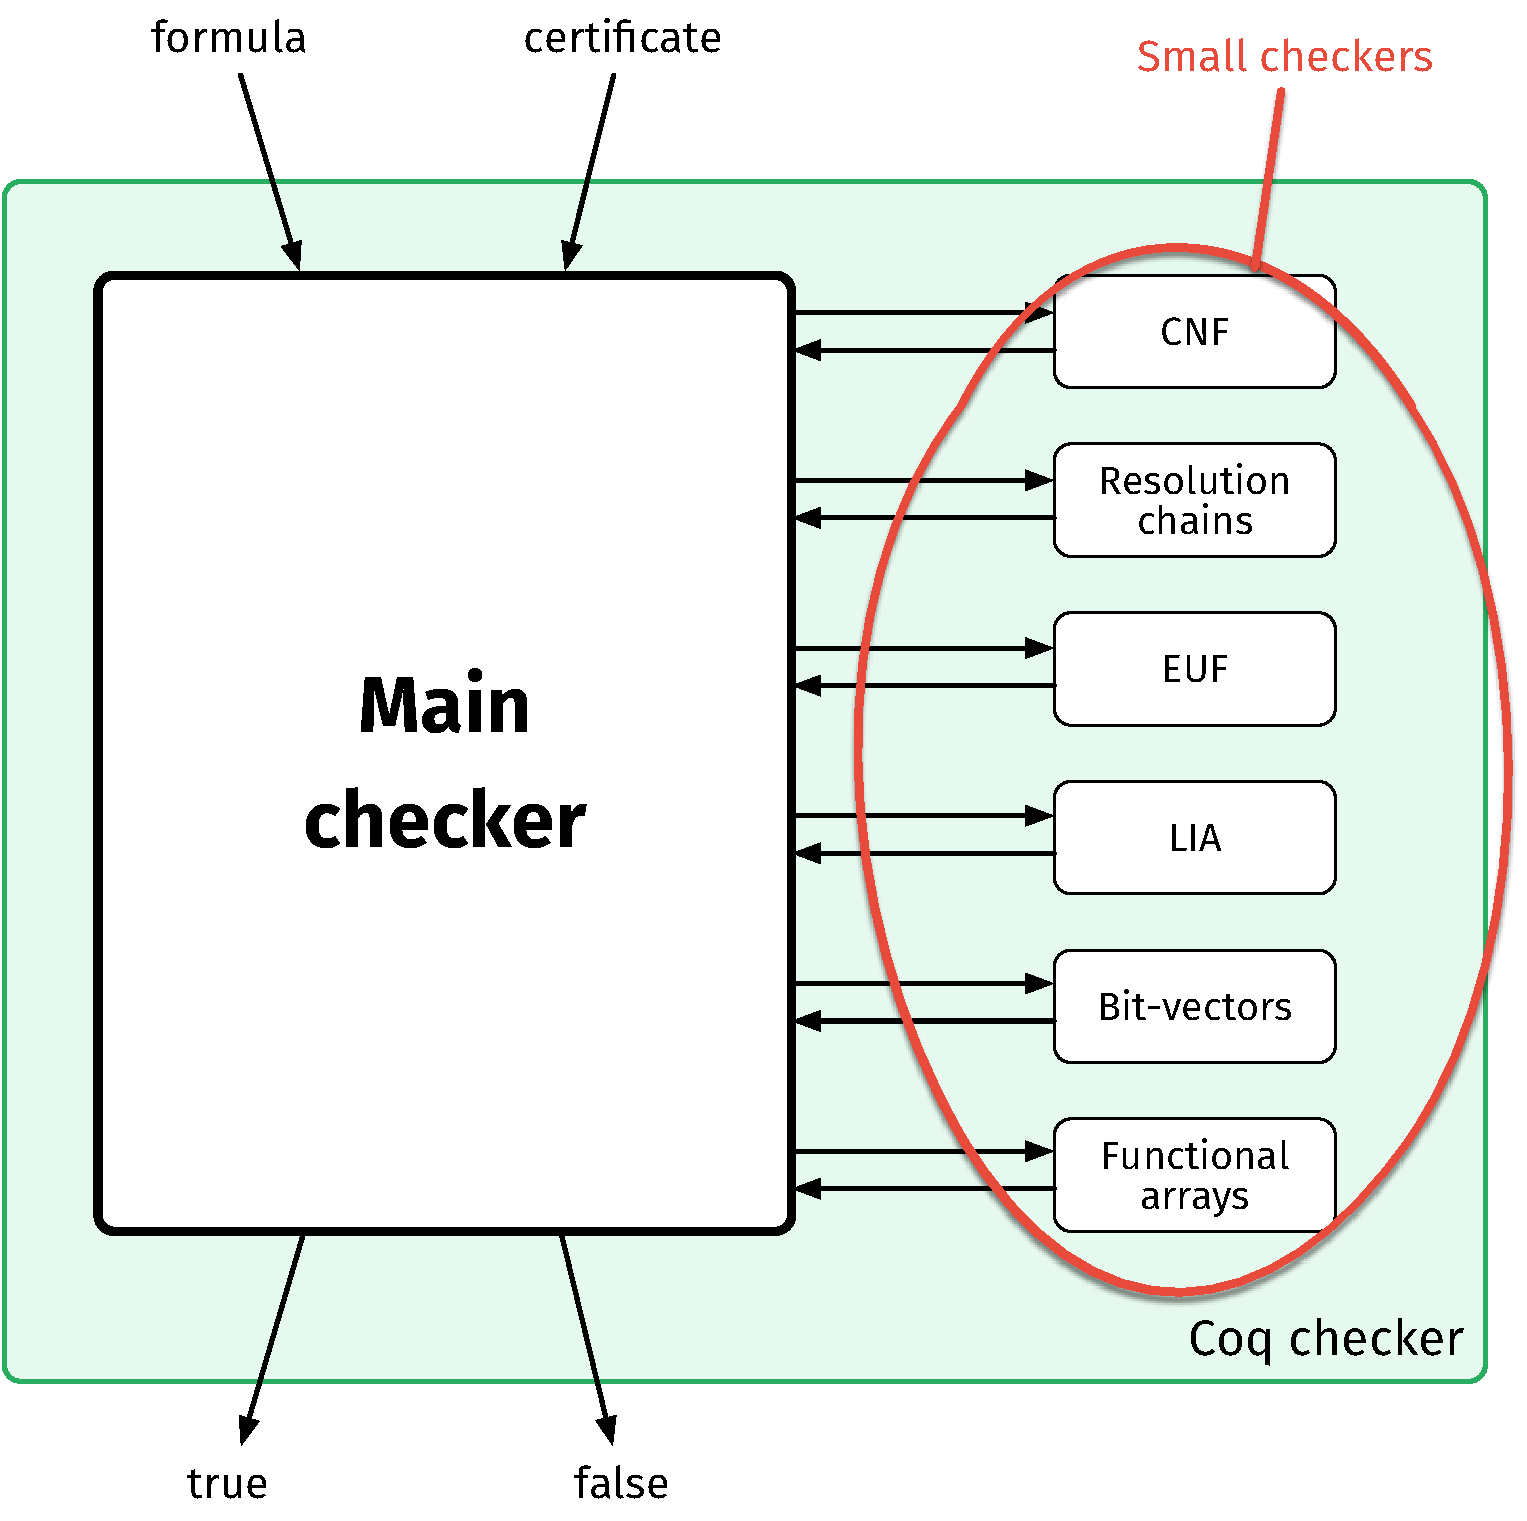
\includegraphics[scale=0.3]{checker}
		\caption{SMTCoq's \texttt{checker}
		shown as the "Main checker" which 
		interacts with various small checkers.}
		\label{fig:checker}
	\end{center}
	\end{figure}
		
	To prove the unsatisfiability of a 
	formula, the SMT solver operates in 
	phases. It converts the formula into
	CNF and performs some simplications
	on it. It then abstracts any theory
	literals into propositional ones 
	and tries to satisfy the abstraction 
	using the SAT solver; it does this
	in a cycle where the theory
	solvers give feedback
	by adding the negation of the 
	satisfying model to the 
	abstraction of the formula if the 
	refinement of the model isn't 
	satisfied by a theory. 
	Each of these phases constitute
	\textit{steps} of the SMT proof
	that SMTCoq has to check. A step
	can modify the current 
	\texttt{state} (representation of 
	the formula) while maintaining 
	its (un)satisfiability. If the 
	initial formula is unsatisfiable, 
	then after running all steps,
	the final \texttt{state} is the 
	empty clause $\bot$. Currently, 
	SMTCoq has steps that perform 
	resolution, conversion of formulas 
	to conjunction normal form (CNF), SMT 
	solver simplifications, and one for 
	each theory. Each step is 
	independently checked by a small 
	checker. Each small
	checker simplifies the  
	\texttt{state} via the step it 
	performs, and the main checker 
	ultimately checks that the input is 
	finally transformed to $\bot$. The 
	architecture of the checker is 
	illustrated in
	Fig.~\ref{fig:checker}.
	
	\subsection{Reflection Lemma}
	\label{sec:refl}
	The process of computational 
	reflection relies heavily on 
	Coq's \textit{conversion rule}.
	Coq's Calculus of Inductive 
	Constructions (CIC) is a 
	$\lambda-$calculus that has a 
	reduction mechanism for terms. The
	reduction rules form a strongly 
	normalizing system. The calculus's
	conversion rule allows a term to 
	have multiple types, as long as the 
	types have the same normal forms. For 
	instance, for some predicate $P$ 
	over natural numbers, a term that 
	has type $P(10)$ also has type 
	$P(5*2)$ and $P(20-10)$. Due 
	to the conversion rule, 
	computations can be used in Coq's 
	reasoning and proof terms can be 
	found simply by computing normal 
	forms of types.
	
	The shallow embedding of formulas in 
	Coq uses types from the 
	Coq standard library along with 
	some custom types. Formulas have a 
	Boolean type, as specified by 
	the \texttt{bool} 
	library~\cite{CoqBool}. The 
	$\mathbb{Z}$ type~\cite{CoqZ}
	from the standard library encodes 
	integer. Additionally, SMTCoq 
	defines its own libraries for 
	bit-vectors and arrays. The shallow 
	embedding for our running example 
	is the formula from the lemma we 
	are trying to prove in Coq
	(Step 1 of fig.~\ref{fig:smtcoqex}):
	\begin{center}
		\texttt{(b \&\& negb c) || (a 
			\&\& negb b) || negb a || c}
	\end{center}	 
	and thus we consider an instantiated
	version of this. SMTCoq deals only 
	with an effectively quantifier-free
	fragment of the SMT solver's logic.
	Even though quantifiers appear in the 
	theorem in Coq (Step 1 of 
	fig.~\ref{fig:smtcoqex}), because
	of the structure of universal 
	quantification where all the variables
	are quantified only in the beginning 
	of the formula, it is straightforward
	to instantiate away the quantifiers
	while negating the formula, and thus
	it suffices to consider the 
	unquantified version.
	
\section{Sledgehammer}
\label{sec:hammer}
	Isabelle~\cite{DBLP:journals/corr/cs-LO-9301106} 
	is an LCF-style system that 
	provides a meta-logic which can be 
	instantiated with other logics.
	Isabelle/HOL~\cite{10.5555/1791547}, 
	one of the most popular Isabelle 
	instantiations, implements a 
	classical higher-order logic. 
	
	Sledgehammer is
	an Isabelle/HOL component that 
	uses external ATPs to enhance 
	Isabelle/HOL with proof 
	automation. Initially, these 
	ATPs only included resolution 
	provers~\cite{10.1007/978-3-642-39799-8_1}.
	The work by Bohme et 
	al.~\cite{bohme} involved 
	extending Sledgehammer to 
	incorporate SMT
	solvers~\cite{Barrett2018} and this 
	work will be our focus for the 
	rest of this section. As with 
	SMTCoq, the SMT solvers integrated
	with Sledgehammer produce a 
	proof object which is 
	then reconstructed within
	Isabelle/HOL by Sledgehammer, 
	using Sledgehammer's own internal 
	ATP --- Metis~\cite{hurd2003d}. The 
	proof object essentially guides 
	the inference steps of the proof 
	within Isabelle/HOL.
	
	Given a conjecture $\Phi$ in 
	Isabelle/HOL, Sledgehammer 
	selects a set of facts 
	$\Gamma$ that might be relevant 
	to proving $\Phi$ and sends
	the formula $\Gamma \land \neg 
	\Phi$ to the SMT solver to check 
	for unsatisfiability. If the SMT 
	solver is able to refute the 
	conjecture (i.e., conclude 
	the unsatisfiability of its 
	negation), it returns 
	a proof. Since Isabelle/HOL 
	implements a higher-order logic 
	(HOL), which 
	is more expressive than 
	the SMT solver's many-sorted
	first order logic (MSFOL),
	the entirety of the formula
	$\Gamma \land \neg \Phi$ may not 
	be understandable to the SMT 
	solver. Parts of the formula,
	however, may be fully 
	first-order (FOL is 
	a subset of HOL). Bohme et al.
	extended Sledgehammer with 
	a translation from higher-order 
	to first-order logic, so that 
	it can reason about the remainder
	of the formula. This translation
	is discussed in the rest of this 
	section.
	
	\subsection{Higher-Order Logic}
	\label{sec:hol}
	In this section, we specify the 
	syntax of higher-order logic 
	and delegate the explanation of 
	semantics to a 
	reference~\cite{10.5555/155278}. 
	HOL consists of 
	types $\tau$ and terms $t$. 
	\begin{align*}
	\tau &:= \alpha\ |\ \kappa^n\ 
	\tau_1 ... \tau_n\\
	t &:= x^{\tau}\ |\ c^{\tau}\ |\ t_1\ t_2\ 
	|\ \lambda x^{\tau}.t
	\end{align*}	
	Types $\tau$ are either type
	variables $\alpha$ or 
	applications of type 
	constructors $\kappa^n$ to 
	$n$ types ($n$ is usually omitted). 
	Particular types of interest are 
	the function type --- formed by 
	applying the arrow type constructor 
	$\to^{2}$ to other types, the 
	Boolean type --- $\texttt{bool}$ 
	(or $\texttt{bool}^0$), the type of 
	natural numbers --- \texttt{nat},
	and integers --- \texttt{int}.
	Terms are typed variables, 
	typed constants, applications 
	of terms to terms, or typed
	$\lambda-$ abstractions. We have
	the usual Boolean constants 
	representing logical connectives
	and quantifiers. For instance, 
	logical negation, 
	$\neg^{\texttt{bool} \to 
	\texttt{bool}}$, universal 
	quantification,
	$\forall^{\alpha \to 
	\texttt{bool} \to \texttt{bool}}$, 
	and polymorphic equality,
	$=^{\alpha \to \alpha 
	\to \texttt{bool}}$. Type 
	annotations for terms are also 
	often omitted when understood
	from context.

	\subsection{Many-Sorted First-Order Logic}
	\label{sec:msfol}
	Many-sorted first-order logic extends
	first-order logic (FOL) with 
	types or sorts. We present the 
	syntax in this section and the 
	semantics are presented in
	\cite{Barrett2018}. Syntactically, 
	the components of MSFOL are sorts 
	$\sigma$, terms $t$, and 
	formulas $\phi$. Sorts are 
	atomic entities that 
	represent types. Function types 
	--- ($\sigma_1$, ..., $\sigma_n$) 
	$\to$ $\sigma$ ---
	and relation types 
	--- ($\sigma_1$, ..., $\sigma_m$)
	are defined over sorts, and 
	are types of functions and 
	predicates below. Terms and 
	formulas are specified as:
	\begin{align*}
		t &:= x^{\sigma}\ |\ 
		f^{(\sigma_1, ..., \sigma_n) \to 
		\sigma}	(t_1, ..., t_n)\\
		\phi &:= \bot\ |\ \neg \phi\ |\ 
		\phi_1 \land \phi_2\ |\ \forall 
		x^{\sigma} . \phi\ |\ t_1 = t_2
		\ |\ P^{\sigma_1,...,\sigma_m}
		(t_1, ..., t_m)
	\end{align*}
	Terms are either sorted variables, 
	or applications of functions to terms.
	Formulas are constants or logical 
	connectives applied to other 
	formulas, quantified formulas, 
	equality over terms, or predicates 
	over terms. Connectives $\lor$, 
	$\to$, $\iff$, and the existential
	quantifier $\exists$ can be 
	specified using the connectives 
	and quantifiers mentioned above.
	
	\subsection{Translation}
	\label{sec:trans}
	Sledgehammer's SMT solver 
	integration (Bohme et al.) performs 
	a translation 
	of HOL formulas to MSFOL formulas.
	$\llbracket\ \rrbracket$
	is the translation function 
	that maps both HOL types and 
	terms to MSFOL sorts and terms,
	respectively.
	The translation is sound --- 
	given a formula 
	$F = \Gamma \land \Phi$ in HOL, if 
	$\llbracket F \rrbracket$ is refutable 
	($\neg \llbracket F \rrbracket$
	is unsatisfiable) in MSFOL, then 
	$F$	is valid in HOL --- but not 
	complete --- if $F$ is valid in 
	HOL, $\llbracket F \rrbracket$ is 
	not necessarily refutable in MSFOL. 
	The translation might not carry over 
	enough information about certain HOL 
	formulas so that the their 
	refutability can be concluded in 
	MSFOL, which is	expected, since HOL 
	is a much more expressive logic than 
	MSFOL. 
	
	Since MSFOL is a subset of 
	HOL, we can see HOL as a 
	composition of 
	MSFOL-equivalent logic 
	and the rest:
	\begin{center}
		HOL = MSFOL-equiv + non-MSFOL 
	\end{center}
	The MSFOL-equiv part of HOL has 
	a straightforward transformation 
	to MSFOL:
	\begin{itemize}
	\item Only nullary type 
		constructors from HOL have
		equivalent MSFOL sorts:
		\begin{center}
			$\llbracket \kappa^{0} 
			\rrbracket = \sigma $
		\end{center}
	\item Applications of 
		Boolean connectives,
		quantifiers, equalities and 
		other predicates (functions 
		returning \texttt{Bool}) to 
		terms have corresponding 
		MSFOL formulas:
		\begin{align*}
			\llbracket False 
			\rrbracket &\cong \bot \\
			\llbracket \neg t \rrbracket 
			&\cong \neg \llbracket t 
			\rrbracket\\
			\llbracket t \land u 
			\rrbracket &\cong \llbracket t 
			\rrbracket \land \llbracket u
			\rrbracket\\
			\llbracket t = u \rrbracket 
			&\cong \llbracket t 
			\rrbracket = \llbracket u
			\rrbracket\\
			\llbracket c^{\tau_1 \to ... 
			\to \tau_n \to \texttt{bool}} 
			t_1 ... t_n \rrbracket &\cong 
			c^{\llbracket \tau_1 \rrbracket, 
			..., \llbracket \tau_n \rrbracket}
			(\llbracket t_1 \rrbracket, ..., 
			\llbracket t_n \rrbracket)\\
			\llbracket \forall x^{\tau}.t 
			\rrbracket &\cong (\forall 
			x^{\llbracket \tau \rrbracket}.
			\llbracket t \rrbracket)
		\end{align*}
	\item Variables and function 
		applications (of return type 
		other than \texttt{bool}), 
		including non-functional 
		constants have MSFOL 
		equivalents.
		\begin{align*}
			\llbracket x^{\tau} 
			\rrbracket &\cong 
			x^{\llbracket \tau \rrbracket}\\
			\llbracket c^{\tau_1 \to ... 
			\to \tau_n \to \tau} 
			t_1 ... t_n \rrbracket &\cong 
			c^{(\llbracket \tau_1 \rrbracket, 
			..., \llbracket \tau_n \rrbracket)
			\to \llbracket \tau \rrbracket}
			(\llbracket t_1 \rrbracket, ..., 
			\llbracket t_n \rrbracket)
		\end{align*}
	\end{itemize}

	The more interesting parts of the 
	transformation deal with 
	translating the non-first-order
	elements of HOL to MSFOL. These 
	include:
	\begin{itemize}
		\item Type variables $\alpha$
		and \textit{compound types} ---
		applications of type constructors
		$\kappa^n$ with $n > 0$ to 
		types.
		\item $\lambda$-abstractions 
		such as $\lambda x. t$.
		\item Variables of functional 
		types and partial applications 
		of functions to arguments are 
		possible in HOL but not in 
		MSFOL. For example, 
		$t^{\tau_1 \to \tau_2 \to 
		\tau}\ t_1$ is a 
		partial application of $t$ 
		which is a variable of type 
		$\tau_1 \to \tau_2 \to \tau$
		to argument $t_1$ (of type 
		$\tau_1$) and this 
		application has type 
		$\tau_2 \to \tau$.
		This is not directly 
		expressible in MSFOL.
	\end{itemize}

	\subsubsection{Monomorphization}
		Recall that HOL types $\tau$ are 
		either type	variables $\alpha$ or 
		applications of type constructors 
		$\kappa^n$ to $n$ types.
		A \textit{monomorphic type} is a
		type without type variables 
		(e.g. $\kappa^0$, $\kappa^1 
		\kappa^0$, and $\texttt{bool}^0 
		\to \texttt{int}^0$ 
		where $\to$ is 
		a type consructor), and 
		a \textit{schematic type} is one 
		with type variables (such as 
		$\alpha \to \texttt{bool}^0$). 
		Monomorphization involves 
		repeatedly instantiating schematic
		terms based on a set of 
		monomorphic terms until a fixed 
		point is reached.
		
		The definition of monomorphization 
		requires a description of 
		\textit{instantiation} of schematic 
		entities w.r.t. 
		monomorphic ones.
		\begin{itemize}
		\item Informally, a monomorphic type 
			$\tau_M$ \textit{matches} a schematic 
			type $\tau_S$ if it can replace the 
			type variables in the schematic 
			type. For example, \texttt{bool} 
			matches $\alpha$; and $\texttt{bool} 
			\to \texttt{int}$ matches 
			$\texttt{bool} \to \beta$
			since \texttt{int} matches 
			$\beta$. Finally, for our running 
			example taken from Bohme et al., 
			${\texttt{bool} \to \kappa}$
			matches $\alpha \to \beta$,
			where $\kappa$ is a monomorphic
			type. 
			
		\item Given a monomorphic constant 
			$c^{\tau_M}$,  if $t^S$ is a 
			schematic term that contains a 
			schematic constant $c^{\tau_S}$ 
			such that $\tau_M$ matches 
			$\tau_S$, then $c^{\tau_M}$ induces 
			a substitution $\sigma$ on $t^S$, 
			and $\sigma(t^S)$ is an instance of 
			$t^S$ w.r.t. to $c^{\tau_M}$. 
			For example, the instance of term
			\begin{center}
				$(\forall f^{\alpha \to \beta},\ 
				x^{\alpha},\ xs^{\texttt{list }
				\alpha}.\ \texttt{apphd }f\ 
				(\texttt{cons }x\ xs) = f\ x)$
			\end{center} 
			w.r.t. constant
			\begin{center}
				$(\lambda x^{\texttt{bool}}.
				\texttt{if }x\texttt{ then }
				a^{\kappa} \texttt{ else }
				b^{\kappa})^{\texttt{bool} \to 
				\kappa}$ 
			\end{center}
			is
			\begin{center}
				$(\forall f^{\texttt{bool} 
				\to \kappa},\ x^{\alpha},\ 
				xs^{\texttt{list }\alpha}. 
				\texttt{ apphd }f\ (\texttt{cons }
				x \ xs) = f\ x)$
			\end{center}
			where the instantiation 
			has turned all occurrences of $f$ 
			in the term from $f^{\alpha \to \beta}$ 
			to $f^{\texttt{bool} \to \kappa}$.
			The following presents some inline, 
			technical preliminaries about 
			the rest of the terms.
			\texttt{list $\alpha$} is a compound,
			polymorphic type of a list of 
			$\alpha$'s where $\alpha$ is a type 
			variable. \texttt{list bool} is the 
			type of lists of Booleans. \texttt{cons} 
			is the list constructor of type 
			$\alpha \to \texttt{list }\alpha \to 
			\texttt{list }\alpha$ and $[\ ]$ is 
			the list constructor for empty lists. 
			For example, the integer list 
			containing $1$, $2$, and $3$ (in that 
			order) is represented as 
			$\texttt{cons }1\ (\texttt{cons }2
			\ (\texttt{cons }3\ [\ ]))$.
			\texttt{hd} is a $\texttt{list}\ 
			\alpha \to \alpha$ function that 
			returns the first element of a list 
			and \texttt{apphd} is an $(\alpha
			\to \beta) \to \texttt{list}\
			\alpha \to \beta$ function that
			takes a function $f$ and a list 
			$l$ as input, and applies $f$
			to the head of $l$ (or, $f\ 
			(\texttt{hd }l)$).
		\item The idea of an instance is 
			extended to terms as follows. If 
			$t^M$ is a monomorphic term, then 
			$\sigma(t^S)$ is an instance of 
			$t^S$ w.r.t. $t^M$, if 
			$\sigma$, the combination of all 
			substitutions induced by the 
			constants in $t^M$ is defined. This 
			instance might still be schematic. For 
			example, since $x^{\texttt{bool}}$ is 
			an instance of $x^{\alpha}$ w.r.t.
			$\texttt{T}^{\texttt{bool}}$, 
			and $xs^{\texttt{list bool}}$ is 
			an instance of 
			$xs^{\texttt{list }\alpha}$ 
			w.r.t. $[\ ]^{\texttt{list bool}}$,
			we can combine the instantiation 
			of the constant in the previous 
			example to obtain that the 
			instantiation of term
			\begin{center}
				$(\forall f^{\alpha \to \beta},\ 
				x^{\alpha},\ xs^{\texttt{list }
				\alpha}.\ \texttt{apphd }f\ 
				(\texttt{cons }x\ xs) = f\ x)$
			\end{center}
			w.r.t. the term
			\begin{center}
				$(\texttt{apphd }(\lambda 
				x.\ \texttt{if }x\texttt{ then }
				a \texttt{ else } b)^{\texttt{bool} 
				\to \kappa}\ (\texttt{cons T}\ 
				[\ ])) \neq a$
			\end{center}
			to be
			\begin{center}
				$(\forall f^{\texttt{bool}
				\to \kappa},\ x^{\texttt{bool}},
				\ xs^{\texttt{list bool}}.\ 
				\texttt{apphd }f\ (\texttt{cons }x
				\ xs) = f\ x)$
			\end{center}
		\item Instantiation can further be 
			extended to sets of schematic 
			terms $S$ and monomorphic terms $M$. 
			An instance of $S$ w.r.t. 
			$M$ is the set $I$ of terms such 
			that each term in $I$ is an instance 
			of some term from $S$ w.r.t. 
			some term from $M$. Since 
			instantiation can produce either 
			monomorphic or schematic terms, $I$
			can be partitioned into either as
			$(I_M, I_S)$.
		\end{itemize}
		Now, we can describe monomorphization.
		\begin{itemize}
		\item A \textit{monomorphization 
			step} for $S$ w.r.t. $M$ maps 
			the pair $(M,S)$ to the pair 
			$(M \cup I_M, S \cup I_S)$.
		\item The complete 
			\textit{monomorphization} of $S$ 
			w.r.t. $M$ is the computation of 
			a least fixed point of 
			monomorphization steps of $S$ 
			w.r.t. $M$.
		\item Given a HOL formula $F$, 
			if $(M, S)$ is the partition of its 
			constituents into monomorphic and 
			schematic terms, then 
			monomorphization of $S$ 
			w.r.t. $M$ yields pair 
			$(M^{\prime}, S^{\prime})$ and we 
			call the conjunction of all terms in 
			$M^{\prime}$ the monomorphization 
			of $F$.
		\end{itemize}
		Thus, using the above examples as 
		instantiation steps, we have that 
		monomorphization translates the formula $F$
		\begin{align*}
			F:\ &(\forall f^{\alpha \to \beta},\ 
			x^{\alpha},\ xs^{\texttt{list }\alpha}.\ 
			\texttt{apphd }f\ (\texttt{cons }x
			\ xs) = f\ x)\ \land\ \\
			&((\texttt{apphd }(\lambda x.\ 
			\texttt{if }x \texttt{ then }a 
			\texttt{ else } b)^{\texttt{bool} 
			\to \kappa}\ (\texttt{cons T}\ [\ ])) 
			\neq a)
		\end{align*}
		to the formula $F^{\prime}$
		\begin{align*}
			F^{\prime}:\ &(\forall 
			f^{\texttt{bool} \to \kappa},\ 
			x^{\texttt{bool}},\ 
			xs^{\texttt{list bool}}.\ 
			\texttt{apphd }f\ (\texttt{cons }x
			\ xs) = f\ x) \ \land\ \\
			&((\texttt{apphd } (\lambda x.\ 
			\texttt{if }x \texttt{ then }a 
			\texttt{ else } b)^{\texttt{bool} 
			\to \kappa}\ (\texttt{cons T}\ 
			[\ ])) \neq a).
		\end{align*}
		\noindent The following are some 
		limitations of this process:
		\begin{itemize}
		\item There have to be monomorphized 
			terms in a formula, to guide the 
			monomorphization process, so it 
			seems like this process would 
			fail with formulas that contain 
			only schematic terms. 
		\item The monomorphization process 
			could be non-terminating. In 
			other words, the first component
			of the pair yielded by 
			monomorphization --- the 
			set of monomorphic terms ---
			could be infinite. For example,
			consider $S = \{c^{\alpha}
			\land c^{\kappa\ \alpha}\}$
			and $M = \{c^{\kappa_0}\}$.
			Now, $\kappa_0$ matches 
			$\alpha$, so the instance
			$c^{\kappa_0} \land 
			c^{\kappa\ \kappa_0}$ is added 
			to $M$ after a monomorphization 
			step. Now, $\kappa\ \kappa_0$
			matches $\alpha$, so the 
			instance $c^{\kappa\ \kappa_0} 
			\land c^{\kappa\ \kappa\ 
			\kappa_0}$ is added to $M$, 
			and so on. Since the proof of a 
			formula, if it existed, would 
			be finite, most monomorphic 
			terms would be irrelevant. 
			Finding the finite subset of 
			necessary monomorphic terms is 
			undecidable~\cite{10.1007/978-3-642-24364-6_7},
			but Bohme et al. use heuristic
			methods to overapproximate
			this set. They limit the 
			number of monomorphization 
			steps and the number of 
			monomorphic terms generated
			with the expectation that 
			monomorphic terms that 
			contribute to proofs 
			are typically generated early 
			in the monomorphization process.
		\item The monomorphization process
			is described as a syntactic 
			process. Semantic steps in 
			the process aren't described, 
			and if it doesn't indeed 
			involve	any semantic pruning of 
			translations, the number of 
			monomorphization steps 
			might be impractically large. 
			For example, from the formula 
			in the running example above ($F$), 
			$x^{\alpha}$ could match 
			$a^{\kappa}$ and be instantiated 
			to $x^{\kappa}$. While 
			syntactically, this would 
			check out, semantically, 
			given that $f^{\alpha \to \beta}$
			is instantiated to 
			$f^{\texttt{bool} \to \kappa}$, 
			and that $f$ is applied to $x$, 
			$x$ has to have type 
			\texttt{bool} and this can be 
			achieved by matching it with 
			$x^{\texttt{bool}}$.
		\item Monomorphization is 
			incomplete and the instantiations 
			are done heuristically. This 
			means that if the SMT solver 
			is not able to prove the 
			monomorphized version of a 
			formula, a different 
			monomorphization could 
			very well be provable. Thus, 
			the monomorphization of a 
			problem would have to be 
			done smartly, and sometimes
			repeated multiple times to 
			be successful. 
		\end{itemize} 
	
	\subsubsection{Lambda-Lifting}
		$\lambda$-abstractions represent 
		anonymous or unnamed functions, 
		which aren't allowed in MSFOL.
		These abstractions are removed
		from HOL formulas by a process 
		called \textit{$\lambda$-lifting}
		which uses a fresh constant as a
		name for the abstraction and adds 
		a quantified formula specifying 
		it's behavior. Concretely,
		\begin{align*}
			\llbracket t[\lambda x^{\tau}.u]
			\rrbracket \cong 
			(t[(\lambda x^{\tau}.u) \mapsto c]
			\land (\forall x^{\tau}.\ c\ x = u))
		\end{align*}
		The notation $t[x]$ represents a 
		term $t$ with a sub-term $x$, 
		and $t[x \mapsto y]$ is the 
		term obtained by substituting all 
		occurrences of $x$ by $y$ in $t$.
		$c$ is specified in MSFOL as an 
		uninterpreted function with sort 
		$\tau \to \kappa$ where $\kappa$ 
		is the sort of $u$. For instance, 
		$(\lambda x^{\texttt{int}}, x + 1)\ 
		5 = 6$
		is translated to $(c\ 5 = 6) \land
		(\forall x^{\texttt{int}}.\ 
		c\ x = x + 1)$. $\lambda-$lifting
		faithfully preserves the 
		semantics of the function, and 
		thus it maintains soundness. 
		Quantified formulas are usually a 
		source of undecidability for SMT 
		solvers, so these lifted formulas 
		contribute to the incompleteness
		of the translation.
		%If the 
		%$\lambda-$ abstraction contains free
		%variables, then they are turned 
		%into additional arguments to $c$.
		
	\subsubsection{Explicit Applications}
		For functional constants 
		occurring multiple times with 
		a variable number 
		of arguments, the minimal 
		number of arguments are 
		considered as the arity of the 
		function, and any additional 
		arguments are expressed 
		explicitly, with the help of a 
		constructor 
		$\texttt{app}^{(\alpha_1 \to 
		\alpha_2) \to \alpha_1 \to 
		\alpha_2}$ that is defined as:
		\begin{center}
			$\texttt{app }t_1\ t_2 = 
			t_1\ t_2$
		\end{center}
		If $c$ is a constant that 
		occurs with at least $n$
		arguments, then 
		occurrences of applications 
		of $c$ are translated as:
		\begin{center}
			$\llbracket c\ t_1\ ...\ t_n
			\ u_1\ ...\ u_m \rrbracket
			\cong \texttt{app}\ (...\ 
			(\texttt{app }(c\ t_1\ 
			...\ t_n)\ u_1)	\ ...)\ u_m$
		\end{center}
		where $m$ could be $0$, in which 
		case there are no applications 
		of \texttt{app}. For example, if 
		$f^{\texttt{int} \to \texttt{int}}$ 
		occurs twice in a formula, once 
		partially applied to no arguments 
		as $f$, and once fully applied as 
		$(f\ 0)$, then since the minimal 
		number of arguments to $f$ is 
		zero, we have:
		\begin{align*}
		\llbracket f \rrbracket &\cong
		f\\
		\llbracket f\ 0 \rrbracket &\cong
		\texttt{app } f\ 0
		\end{align*}
		
		\texttt{app} is a higher-order 
		function so both the function 
		($f$ in the above example) and 
		\texttt{app} have to be encoded 
		in the SMT solver as constructors.
		This can also be done using arrays 
		which are essentially functional 
		types which can be passed
		around, since arrays in 
		SMTLIB~\cite{BarFT-SMTLIB} (the 
		standard for SMT solvers)
		can have any index and value types, 
		and map elements of the index type 
		to the value type. Bohme et al. 
		don't specify what technique 
		they use to encode the 
		\texttt{app} constructor.
		
		Using the \texttt{app} constructor
		for partially applied interpreted 
		constants in MSFOL, such as 
		logical connectives, would result 
		in terms that aren't well-typed.
		These are $\eta-$expanded and 
		then $\lambda-$lifted. For example, 
		for the partially applied 
		conjunction ($\land$, used as prefix 
		here), a partial application is 
		translated as follows.
		\begin{align*}
			\llbracket t [\land\ x] 
			\rrbracket &\cong \llbracket 
			 t[\lambda y.\ \land\ x\ y]
			\rrbracket&(\eta-expansion)\\
			&\cong t[c]  \land (\forall y.\ 
			c\ y = \land\ x\ y) &(\lambda-lifting)
		\end{align*}
		
	\subsubsection{Erasure of Compound Types}
		A type constructor $\kappa^n$ with 
		$n > 0$ is applied to $n$ types 
		$\tau_i$. After monomorphization, 
		each $\tau_i$ is monomorphic, so 
		$\kappa^n\ \tau_1\ ...\ \tau_n$ 
		is a monomorphic, compound type. It
		is represented as a fresh nullary 
		type constructor $\kappa_0^n$ with 
		the same interpretation as 
		$\kappa^n\ \tau_1\ ...\ \tau_n$, 
		which can now be represented in 
		MSFOL.
		\begin{center}
			$\llbracket \kappa^n\ 
			\tau_1\ ...\ \tau_n \rrbracket
			\cong \kappa_0^n$
		\end{center}
		Some examples are:
		\begin{align*}
			\llbracket \texttt{bool} \to
			\kappa \rrbracket &\cong \kappa_1\\
			\llbracket \texttt{list\ bool}
			\rrbracket &\cong \kappa_2
		\end{align*}
		At the time of writing of Bohme et al.,
		SMT solvers didn't support sorts 
		parameterized by other sorts, but they 
		support them now, and these can be 
		used to encode compound types.
		
		While this is a straightforward
		translation step syntactically, 
		notice that SMT solvers need 
		extra help via premise selection 
		to solve constraints involving 
		these types. Integers are 
		axiomatized in the SMT solver as 
		the theories of linear and 
		non-linear integer arithmetic, and 
		Isabelle/HOL integers are made to 
		correspond to these in the translation, 
		so when a formula containing 
		integers is sent to the SMT solver, 
		it can perform integer reasoning. 
		However, SMT solvers have no 
		axiomatization of, say, lists 
		of Booleans. It is crucial that when 
		\texttt{list bool} is 
		translated to $\kappa_2$, the 
		premise selector of sledgehammer
		selects the right lemmas about 
		Boolean lists to give to the 
		SMT solver so it can reason 
		about them. So in this step, 
		completeness depends heavily on 
		premise selection.
		
	\subsubsection{Interpreted and Uninterpreted Constants}
		As mentioned in the previous section,
		certain types in Isabelle/HOL correspond
		to certian sorts in the SMTLIB standard.
		Bohme et al. exploit the axiomatizations 
		of these sorts by translating constants 
		of these types from HOL to the 
		corresponding MSFOL constants - these 
		include linear arithmetic constants over 
		integers and reals and bit-vector 
		arithmetic. They even use the SMTLIB 
		theory of algebraic 
		datatypes~\cite{BarST-PDPAR-06} to 
		encode inductive types from Isabelle/HOL
		such as lists. This allows the SMT solver
		to rely on the decision procedures for 
		these theories and not just the premises
		provided by Sledgehammer, to prove the 
		conjecture. 
		
		The rest of the constants are 
		translated as uninterpreted constants, 
		and this is a source of 
		incompleteness --- the SMT solver only 
		knows as much about an uninterpreted 
		constants as the additional constraints 
		(premises) will tell it. If the premise 
		selector of Sledgehammer doesn't capture 
		the constraints needed to prove something
		about an uninterpreted constant, the SMT 
		solver will not be able to prove it.
		Even with interpreted constants, if the 
		constants belong to an undecidable theory,
		the SMT solver will not necessarily be 
		able to prove it.
		
\bibliographystyle{abbrv}
\bibliography{bib2new}

\end{document}